% !TeX root = ../thuthesis-example.tex

\chapter{国内外研究现状}\label{chapter2}
\section{引言}
本章节对研究内容相关的文献进行了调研,对研究现状进行了阐述、分析和总结。
同时为了方便理解研究内容、方便阅读,也对涉及到的一些相关的背景知识进行了介绍。
\section{时间序列预测方法}
  针对章节\ref{goal}中提出的第一个研究目标:训练出准确度能满足实际应用需求的时间序列预测模型。
  这里调研了常用的时间序列预测的模型和方法,和一些提高预测效果的手段,
  同时也对不同模型的特点进行了分析。
\subsection{时间序列预测常用模型}

  处理时间序列的常用方法包括两类,
  一类是传统的统计模型例如ETS和ARIMA,第二类是基于深度神经网络。

  基于深度神经网络的模型预测方法近年来越来越具有竞争力。
  传统的统计学模型依然具有其兼顾准确率高、模型相对简单、鲁棒性好、高效等优势。
  然而,更复杂,更高维度和以及包含噪声的现实世界中的时间序列数据
  无法用带有参数的解析方程来描述,因为动力学太复杂且未知,
  传统浅层方法因为只包含一个小的非线性操作的数量,
  没有能力准确地模拟这种复杂的数据。
  从未标记数据中学习特征的优点是可以利用丰富的未标记数据,
  并且可以学习比手工制作的特征更好的特征。
  这两个优点都减少了对数据专业知识的需求。

  近年来,在时间序列预测领域,也有关于标准框架的基础工作支持深度学习在时间序列预测问题上的发展。
  出现了为时间序列预测研究设计的
  GluonTS开源框架\cite{DBLP:journals/corr/abs-1906-05264}。

  \begin{figure}
    \centering
    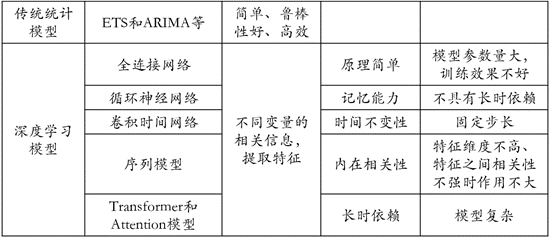
\includegraphics[width=\linewidth]{figures/预测典型模型.png}
    \caption{应用于时间序列预测的典型模型类型及其特点总结}
    \label{tab:prediction models}
  \end{figure}
  常用的深度神经网络包括循环神经网络(如LSTM和GRU)、
  序列模型、卷积神经网络、Transformer和Attention模型。
  M4竞赛结果表明\cite{MAKRIDAKIS202054},
  准确率最好的模型都结合了传统统计模型和深度学习模型,
  或多种深度学习模型。在时间序列预测问题上,
  没有哪一种绝对优势的模型,各种模型都有其结构上的优势特点。
  不同模型的优势特点如表\ref{tab:prediction models}。

  \paragraph{循环神经网络在时间序列预测问题上的应用效果及问题}~{}

    DeepAR提出基于LSTM的时间序列概率自回归预测模型
    \cite{salinas2020deepar},
    用LSTM模型建模未来时间步中的贝叶斯模型。
    近年提出的模型中,结合了指数平滑方法的混合RNN模型\cite{smyl2020hybrid}
    在M4预测竞赛中成为最终的优胜模型\cite{MAKRIDAKIS202054}。
    循环神经网络由于其独特的记忆机制\cite{hewamalage2021recurrent},
    一直都是处理时间序列问题的最通用选择之一,
    常用的模型结构如长短时记忆LSTM和门控循环单元GRU。

    GRU-ODE-Bayes网络\cite{de2019gru}构建了一个连续版本的门控循环神经网络,
    利用贝叶斯的方法更新,在多项任务中取得了很好的效果。

    但是循环神经网络也有其缺点,比如对并行训练的支持不好、
    不能捕捉过长的时序依赖关系等。
    所以人们也一直没有放弃对其他网络结构在时间序列预测问题上的探索。

  \paragraph{序列模型能有效捕捉相关性及构造时变模型}~{}

    常见的序列模型一般包括编码器和解码器两部分。
    能够捕捉时间序列数据之间的相关性。
    目前效果较好的序列模型是由多个RNN组成。

    \begin{figure}
      \centering
      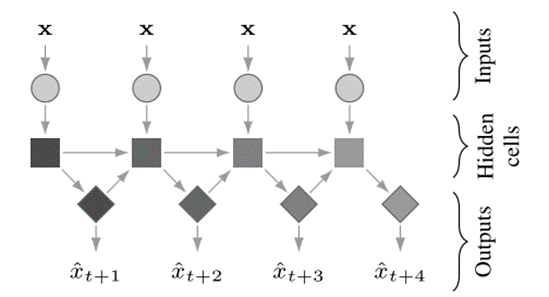
\includegraphics[width=0.8\linewidth]{figures/ForecastsNet 网络结构.png}
      \caption{ForecastsNet 网络结构}
      \label{tab:ForecastsNet}
    \end{figure}

    ForecastNet\cite{dabrowski2020forecastnet}中采用Dense连接的方式,
    如图\ref{tab:ForecastsNet}所示,
    实现了时变的模型结构,同时通过交错输出的方式,
    有效地缓解了梯度消失的问题,
    在多步的时间序列预测问题上得到了不错的准确度。  
  
  \paragraph{应用于时间序列预测的卷积神经网络}~{}
  
    \begin{figure}
      \centering
      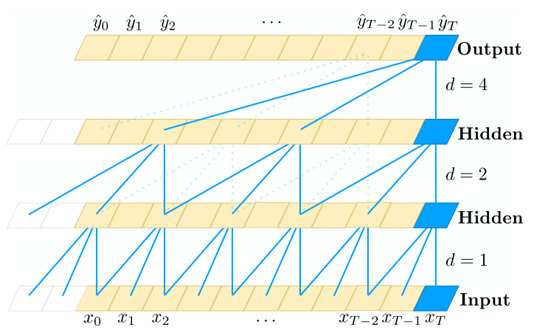
\includegraphics[width=0.8\linewidth]{figures/TCN空洞卷积结构.png}
      \caption{TCN空洞卷积结构}
      \label{tab:TCN}
    \end{figure}
    早在上个世纪80年代末,卷积的结构就被应用于序列问题上
    \cite{lecun1989backpropagation}。
    卷积神经网络通过卷积和参数共享来实现位移不变性的效果\cite{amari2003handbook},
    能够应用在时间序列模型上,具有时间不变性的特性。
    在建模序列数据问题上,通过多个评价系统\cite{chung2014empirical}的测试,
    达到了相当不错的效果,
    明显优于循环神经网络\cite{binkowski2018autoregressive}。
    卷积神经网络相比循环神经网络,
    结构上支持并行,计算速度方面能够得到有效地保证。
    也有相关工作\cite{shi2015convolutional}结合了卷积神经网络和循环神经网络,
    用卷积层替换了长短时记忆网络中原有的全连接层。

    以Temporal Convolution Networks (TCN) 为代表的更先进的卷积神经网络,
    结合了更大的卷积范围和残差跳跃连接,在序列建模任务的训练上,
    取得了很好的效果\cite{bai2018empirical,pascanu2013construct}。
    TCN应用了空洞卷积的卷积结构,
    如图 2中的感受野足够大,能够捕捉序列中的长时依赖信息,
    而且利用了残差连接,有效地提升了模型的准确率。
  
\subsection{提高预测效果方法}
  \paragraph{经验模态分解}~{}

    经验模态分解(Empirical Mode Decomposition, EMD)
    方法被认为是自2000年来,以傅立叶变换为基础的线性和稳态频谱分析的一个重大突破。
    
    对于非线性数据尤其是非平稳数据,直接处理会非常难,
    但是这类数据就比较适合用经验模态分解来处理,
    经验模态分解在这类数据的处理上会具有明显的优势。
    
    经验模态分解也常常会被用在信噪比低的数据上提升数据的信噪比。
\section{对时间序列模型的训练加速}
  \subsection{模型训练加速方法研究现状}
  时间序列模型的训练速度严重制约了深度学习在时间序列上的应用。
  模型的训练加速一般有特征、样本、模型几个方向的思路。对特征进行降维、筛选有效样本、
  利用多级模型在保证准确率的情况下降低使用的模型的复杂度。

  另外图像领域对训练加速的研究对时间序列模型也有一定的借鉴意义。
  为了保证阐述的完整性,这里列出了其他的一些可以参考的图像问题加速的方法。
  以常用的卷积神经网络为例,常用的加速方法包括:
  (1)张量分解,(2)低精度的运算和其他量化方法,(3)对大网络进行剪枝,
  (4)用Teacher-Student方法通过训练小网络得到大网络,
  (5)设计高效的网络结构,用启发式的方法找到最精简的网络结构,
  (6)网络结构的自动搜索等\cite{lebedev2018speeding}。
  近年来,研究者们将模型训练的效果提升和过程加速的注意力转移到重要性采样上来。

  \subsection{筛选有效样本(重要性采样)}
  重要性采样(Importance Sampling)是统计学中估计某一分布性质时使用的一种方法。
  该方法从与原分布不同的另一个分布中采样,而对原先分布的性质进行估计。

  重要性采样被应用于提升凸优化问题的随机优化方法的收敛速度上,
  例如构造核分类器\cite{bordes2005fast}、
  用随机过程优化正则化损失\cite{zhao2015stochastic}等。
  另外一方面,在深度神经网络领域,
  样本筛选的方法也被应用于解决困难样本的处理问题,
  例如在嵌入学习问题中\cite{wu2017sampling},也被应用于解决样本不平衡的问题。

  深度神经网络花费了很多重复的计算量在处理很容易拟合的样本上,
  这些样本在训练一段时间后,就能被忽略掉,并不会影响最终的模型效果,
  在训练过程的某些时间开始忽略这样的样本,能大大地节省模型优化的计算量。
  也就是说,在训练过程中,不同的样本对收敛过程起到的作用效果是不一样的,
  很多样本在很少的几个轮次之后就能被很好地分类或者拟合,通过对样本的筛选,
  能够在较少影响准确率的情况下有效地加速训练过程。

  近年来的一些工作表明\cite{needell2014stochastic},
  重要性采样的方法的加速原理是降低随机梯度下降过程中梯度估计的方差,
  最优的采样分布应该和样本的梯度范数成正比。
  所以重要性采样一般围绕梯度范数展开,但是由于梯度范数的计算复杂度过高,
  另外一种常用的思路是通过训练过程的损失来对梯度范数进行拟合,
  从而计算样本重要性。
  通过损失来计算样本重要性的方法通常有很多超参数需要调优,
  并且对梯度范数拟合得不够。
  为了探索一种更好的训练数据选择策略,
  包括课程学习(curriculum)和自步学习(Self-paced Learning)
  在内的先前工作都采用了简单的启发式规则,例如打乱序列长度来训练语言模型,
  或放弃损失值大于手动定义的阈值的训练样本。
  这种人为定义的规则在一定程度上受限于某些任务,
  不能推广到更广泛的学习场景,
  因为不同的学习任务可能会产生不同的最佳数据选择规则,
  甚至一个学习任务可能也需要具有各种属性的数据才能在不同的训练阶段进行优化。

  Yang Fang等人应用强化学习的方法来选取样本\cite{fan2016neural}。
  通过强化学习来设计一个训练数据的过滤器(Neural Data Filter, NDF)插入到网络输入层之前,
  在训练的过程中动态筛除一部分对训练益处不大的数据,从而减少训练数据量。
  该方法有两个直观的原则:一方面,数据选择策略应该是通用的,
  这样就可以自然地将其应用于不同的学习场景,
  而无需进一步的人工设计。 另一方面,该策略应具有前瞻性,
  因为它在训练的每个步骤中的选择都会带来更好的长期回报,
  而不是暂时适应当前阶段。

  NDF的基本工作流程是:给定当前训练中的网络的状态和当前mini-batch数据的状态(states)   ,
  输出一组动作(action) ,  是一个0,1向量,
  它的维度和mini-batch的大小相同,
  每个元素代表了mini-batch中对应的数据是否应该被剔除。
  利用强化学习的方法来建立过滤器的过程包括以下几个步骤,首先通过现有的采样的policy,
  输入当前的模型状态和待采样样本状态,输出采样的结果,然后将样本输入模型中,
  得到实际的梯度下降的效果的Reward,继而用Reward对采样的policy进行优化。

  \subsection{重要性采样介绍}

  \paragraph{蒙特卡洛积分}~{}

  提到重要性采样首先要介绍蒙特卡洛积分的概念。

  蒙特卡洛是一类算法的总称,是用随机抽样和统计模拟的方法,来进行数值计算。
  它的基本做法是,做大量重复实验来统计频率,
  根据伯努利大数定律,当样本数足够多时,频率会无限接近于概率,
  所以理所当然,可以通过频率来估计概率。

  对于求解积分$\int_a^b f(x)dx$,经典的方法是我们需要找出$f(x)$的原函数$F(x)$。
  但是,在求积分的过程中,积分的原函数在很多情况下都不是很容易获得,那么我们就无法应用经典的求解积分的方法。

  蒙特卡洛积分是蒙特卡洛算法的具体应用。
  蒙特卡洛方法在估计$\int_a^b f(x)dx$积分时,将其表示为一个均匀随机变量的期望,如下,
  \begin{equation}
      \theta=\int_a^b f(x)dx = (b-a)\int_a^b f(x) \frac{1}{b-a}dx=(b-a)E(f(X)), X\sim U(a,b)
  \end{equation}
  其中$U(a,b)$代表在[a,b]之间的均匀分布。从而可以通过如下算法来得到积分估计的结果:
  \begin{enumerate}
      \item 从分布$U(a,b)$中产生i.i.d样本$x_1,x_2,x_3,...,x_n$;
      \item 计算$f(X)$期望的估计值$\overline{f(X)}=\frac{1}{n}\sum_{i=1}^{n} f(x_i)$;
      \item 得到$\hat{\theta}=(b-a)\overline{f(X)}$。
  \end{enumerate}
  容易得到,估计值$\hat{\theta}$的期望和方差分别为,

  $E\hat{\theta}=\theta$,
  $Var(\hat{\theta})=(b-a)^2 Var(\overline{f(X)})=\frac{(b-a)^2}{n}Var(f(X))$

  但是基于均匀分布的估计方法,不能应用于无穷积分的估计,
  而且当被积函数在积分区间上的分布不是很均匀时,抽样的效率会比较低。

  \paragraph{重要性采样}~{}

  前面的蒙特卡洛积分经典计算方法采用均匀分布作为加权函数,会有抽样效率的问题,
  重要性采样就是一种利用合理的加权函数,提高抽样样本效率的计算方法。
  和经典的计算方法相比,重要性采样的加权函数不再是均匀分布。
  设随机变量$X$的概率密度函数是$g(x)$。记$Y=\frac{f(x)}{g(x)}$
  \begin{equation}
      \theta=\int_a^b f(x)dx = \int_a^b \frac{f(x)}{g(x)}g(x)dx=EY
  \end{equation}
  再通过简单的蒙特卡洛积分方法估计$EY$:
  \begin{equation}
      \hat{\theta}'=\hat{EY}=\frac{1}{n}\sum_{i=1}^{n}y_i=\frac{1}{n}\sum_{i=1}^{n}\frac{f(x_i)}{g(x_i)}
  \end{equation}
  此处$x_1,x_2,x_3,...,x_n$为从g(x)中抽取的样本。
  用这个方法估计的参数的方差为
  $Var(\hat{\theta}')=Var(Y)/n$。当$Y$为常数时方差为0。
  所以,$f(x)$的选择目标应该是尽量接近$g(x)$。

  % \subsection{优化理论} % Todo